%
% Zusammenfassung Communication Networks D-ITET
% ===========================================================================
% Author:			Marco Dober
% Version:			0.1
% Last changed: 	19.02.2019	
% ---------------------------------------------------------------------------

\documentclass[a4paper, fontsize=8pt, landscape, DIV=1]{scrartcl}
\usepackage{lastpage}
\usepackage{hyperref}
\usepackage{graphicx}
% Include general settings and customized commands
%
% General packages and settings
% ===========================================================================
% Author:			Silvano Cortesi (cortesis@student.ethz.ch)
% Version:			1.2
% Last changed:		03.01.2018
%
% ---------------------------------------------------------------------------




\usepackage[german]{babel} %choose your language \usepackage[german]{babel}
%\usepackage[T1]{fontenc}
\usepackage[utf8]{inputenc}
\usepackage{fancyhdr}
%\usepackage{lastpage}
%\usepackage{lmodern}
\usepackage{enumerate}
%\usepackage{float} % for positioning of figures
\usepackage[landscape, margin=1cm]{geometry}
\usepackage[dvipsnames]{xcolor}
\usepackage{pdfpages}


%% Math %%
\usepackage{todonotes}
\usepackage{amscd}
\usepackage{blindtext}
\usepackage{enumitem}
\usepackage{multicol}
\usepackage{parskip}
\usepackage{empheq}
\usepackage{amsmath}
\usepackage{amsfonts}
\usepackage{amssymb}
\usepackage{amsthm}
%\usepackage{dsfont}
%\usepackage{esint} % provides \oiint
\usepackage{mathrsfs}
%\usepackage{trfsigns}
%\numberwithin{equation}{subsection}
%\usepackage{numprint}

%% Graphics & Charts %%
\usepackage{graphicx}
%\usepackage{pdfpages}
%\usepackage{booktabs}
\usepackage{array}
%\usepackage{paralist}
%\usepackage{framed}
%\usepackage{trfsigns}
\usepackage{tikz}
%\usepackage[lofdepth,lotdepth]{subfig}
%\usepackage{tikz}  %Graphen zeichnen
%\usetikzlibrary{decorations.pathmorphing}
%\usetikzlibrary{arrows.meta,arrows}
%\usepackage{pgfplots}
%% General Settings %%
%\setlength{\parindent}{0px}
%\setkomafont{captionlabel}{\normalfont\bfseries}

%\pagestyle{fancy}
%\lfoot{\tiny \today}
%\rfoot{\thepage\  / \pageref{LastPage}}
%\cfoot{}
%\renewcommand{\footrulewidth}{0.4pt}

%% provides command \uline{} for underlining words
%\usepackage{ulem}

%% colour headings
%\usepackage{color}
%\definecolor{bluen}{cmyk}{1,0.5,0,0}
%\definecolor{bloodorange}{cmyk}{0,.92,1,.2}
%\addtokomafont{section}{\color{bloodorange}}
%\addtokomafont{subsection}{\color{bloodorange}}
%\addtokomafont{subsubsection}{\color{bloodorange}}
%\addtokomafont{paragraph}{\small\color{bloodorange}}
%\addtokomafont{subparagraph}{\small\color{bloodorange}}

%% Signs & Special Formating %%
%\usepackage{ulem} %normalem: \emph{Text} is italic again.
%\usepackage{multicol,multirow}
%\usepackage{tabularx}
%\usepackage{stackrel}
%\usepackage{makeidx}
%\usepackage{mparhack} % bessere margiale bei seitenumbruch

% make document compact
\usepackage[compact]{titlesec}
\titlespacing{\section}{0pt}{*0}{*0}
\titlespacing{\subsection}{0pt}{*0}{*0}
\titlespacing{\subsubsection}{0pt}{*0}{*0}

\parindent 0pt
\pagestyle{empty}
\setlength{\unitlength}{1cm}
\setlist{leftmargin = *}

%include also newer PDF
\pdfminorversion=6

% Set the color of your style
% Avaiable are: Apricot, Aquamarine, Bittersweet, Black, Blue, blue, BlueGreen, BlueViolet, BrickRed, Brown, BurntOrange, CadetBlue, CarnationPink, Cerulean, CornflowerBlue, Cyan, Dandelion, DarkOrchid, Emerald, ForestGreen, Fuchsia, Goldenrod, Gray, Green, GreenYellow, JungleGreen, Lavender, ... (more at: http://en.wikibooks.org/wiki/LaTeX/Colors)
\def\StyleColor{MidnightBlue}

%
% General commands
% ===========================================================================
% Author:			Silvano Cortesi (cortesis@student.ethz.ch)
% Version:			1.2
% Last changed:		03.01.2018
%
% ---------------------------------------------------------------------------

%..ROEMISCHE_ZAHLEN
	\newcommand{\Roe}[1]{\uppercase\expandafter{\romannumeral #1 }}

%..ZAHLENMENGEN
	\newcommand{\N}{\mathbb{N}}
	\newcommand{\Z}{\mathbb{Z}}
	\newcommand{\Q}{\mathbb{Q}}
	\newcommand{\R}{\mathbb{R}}
	\newcommand{\real}{\R}
	\newcommand{\C}{\mathbb{C}}
	\newcommand{\complex}{\C}
	\newcommand{\0}{\mathbb{O}}
	\newcommand{\F}{\mathbb{F}}
	\newcommand{\K}{\mathbb{K}}
    \newcommand{\angstrom}{\textup{\AA}}
    
%..PFEILE
	\renewcommand{\leadsto}{\Longrightarrow}
	\newcommand{\leftrightleadsto}{\Longleftrightarrow}

%..VEKTOREN
	\newcommand{\Ul} {\underline}
	\newcommand{\vEx} {\vec{e}_x}
	\newcommand{\vEy} {\vec{e}_y}
	\newcommand{\vEz} {\vec{e}_z}
	\newcommand{\vEq} {\vec{e_1}}
	\newcommand{\vEw} {\vec{e_2}}
	\newcommand{\vEe} {\vec{e_3}}
	\newcommand{\transpose} {^{\text{T}}}
	\newcommand{\vect}[1]{\boldsymbol{#1}}
	
%..MATRIX
    \newcommand{\MATR}[1]{ \displaystyle \left( \begin{matrix} #1 \end{matrix} \right)}
    \newcommand{\MATRABS}[1]{ \displaystyle \left| \begin{matrix} #1 \end{matrix} \right|}

%..GRAPHICS
  \newcommand{\cgraphic}[2]{\begin{center}\includegraphics[width=#1\columnwidth,keepaspectratio]{#2}\end{center}}
  
%..FONTS AND LETTERS
  \newcommand*{\rom}[1]{\uppercase\expandafter{\romannumeral #1\relax}}

%..KOMPLEXE ZAHLEN
	\renewcommand{\Re}{\text{Re}\,}
	\renewcommand{\Im}{\text{Im}\,}

%..OPERATOREN
	\DeclareMathOperator{\grad}{grad}
	\renewcommand{\div}{\text{div}\,}
    	\DeclareMathOperator{\rot}{rot}
    	\DeclareMathOperator{\divg}{div}
    	\DeclareMathOperator{\Tr}{Tr}
    	\DeclareMathOperator{\const}{const}
	\DeclareMathOperator{\imag}{i}
	\newcommand{\Lapl}{\hbox{\footnotesize{$\Delta$}}}

%..DIFFERENTIALRECHNUNG
	\newcommand{\Dx} {\,\mathrm{d}}
	\newcommand{\abl}[1] {\frac{\mathrm{d}}{\mathrm{d}#1}}
	\newcommand{\Abl}[2] {\frac{\mathrm{d}#1}{\mathrm{d}#2}}
	\newcommand{\ablq}[1] {\frac{\mathrm{d^2}}{\mathrm{d}#1^2}}
	\newcommand{\Ablq}[2] {\frac{\mathrm{d^2}#1}{\mathrm{d}#2^2}}
	\newcommand{\pabl}[1] {\frac{\partial}{\partial#1}}
	\newcommand{\pablq}[1] {\frac{\partial^2}{\partial#1^2}}
	\newcommand{\Pabl}[2] {\frac{\partial#1}{\partial#2}}
	\newcommand{\Pablq}[2] {\frac{\partial^2#1}{\partial#2^2}}

%..INTEGRALRECHNUNG
	\newcommand{\dint}{\displaystyle{\int}}
	\newcommand{\intab}{\int^b_a}
	\newcommand{\intinf}{\int_{-\infty}^\infty}
	\newcommand{\dintab}{\displaystyle{\int^b_a}}
	\newcommand{\dintpi}{\displaystyle{\int^{\pi}_{-\pi}}}
	\newcommand{\dintzpi}{\displaystyle{\int^{2\pi}_{\mbox{-}2\pi}}}
	\newcommand{\dA}{\hspace{4pt}\mathrm{d}A}
	\newcommand{\dx}{\hspace{4pt}\mathrm{d}x}
	\newcommand{\dy}{\hspace{4pt}\mathrm{d}y}
	\newcommand{\dz}{\hspace{4pt}\mathrm{d}z}
	\newcommand{\dr}{\hspace{4pt}\mathrm{d}r}
	\newcommand{\ds}{\hspace{4pt}\mathrm{d}s}
	\newcommand{\dS}{\hspace{4pt}\mathrm{d}S}
	\newcommand{\dt}{\hspace{4pt}\mathrm{d}t}
	\newcommand{\dm}{\hspace{4pt}\mathrm{d}m}
	\newcommand{\dk}{\hspace{4pt}\mathrm{d}k}
	\newcommand{\dl}{\hspace{4pt}\mathrm{d}l}
	\newcommand{\du}{\hspace{4pt}\mathrm{d}u}
	\newcommand{\dv}{\hspace{4pt}\mathrm{d}v}
	\newcommand{\dV}{\hspace{4pt}\mathrm{d}V}
	\newcommand{\dphi}{\hspace{4pt}\mathrm{d}\varphi}
	\newcommand{\domega}{\hspace{4pt}\mathrm{d}\omega}
	\newcommand{\dvarsigma}{\hspace{4pt}\mathrm{d}\varsigma}
	\newcommand{\dtau}{\hspace{4pt}\mathrm{d}\tau}
	\newcommand{\dtheta}{\hspace{4pt}\mathrm{d}\vartheta}
	\newcommand{\dmu}{\hspace{4pt}\mathrm{d}\mu}
	\newcommand{\dxi}{\hspace{4pt}\mathrm{d}\xi}
	\newcommand{\deta}{\hspace{4pt}\mathrm{d}\eta}
	\newcommand{\dvecl}{\hspace{4pt}\mathrm{d}\vec{l}}
	\newcommand{\dvecS}{\hspace{4pt}\mathrm{d}\vec{S}}

%..LIMES
    \DeclareMathOperator{\limni}{\lim\limits_{n\to\infty}}
    \DeclareMathOperator{\limxi}{\lim\limits_{x\to\infty}}
    \DeclareMathOperator{\limho}{\lim\limits_{h\to0}}
    \newcommand{\limxai}[1]{\ensuremath{\lim\limits_{x\to #1}}}

%..SUMMEN
    \DeclareMathOperator{\sumni}{\sum_{n=0}^{\infty}}
    \newcommand{\sumnia}[1]{\ensuremath{\sum_{n=#1}^{\infty}}}


%..PARTIELLE ABLEITUNG
    \DeclareMathOperator{\partf}{\dfrac{\partial f}{\partial x}}
    \newcommand{\partfo}[1]{\ensuremath{\dfrac{\partial f}{\partial #1}}}
    \newcommand{\parto}[1]{\ensuremath{\dfrac{\partial }{\partial #1}}}
    \newcommand{\partt}[2]{\ensuremath{\dfrac{\partial^2 }{\partial #1\partial #2}}}
    \newcommand{\partq}[1]{\ensuremath{\dfrac{\partial^2 }{\partial #1^2}}}


%..ENUMERATION
    \newenvironment{abc}{\begin{enumerate}[(a)]}{\end{enumerate}}
    \newenvironment{cabc}{\begin{compactenum}[(a)]}{\end{compactenum}}
    \newenvironment{romanenum}{\begin{enumerate}[i.]}{\end{enumerate}}
    \newenvironment{cromanenum}{\begin{compactenum}[i.]}{\end{compactenum}}

%..FUNCTIONS
    \DeclareMathOperator{\arsinh}{arsinh}
    \DeclareMathOperator{\arcosh}{arcosh}
    \DeclareMathOperator{\artanh}{artanh}
    \DeclareMathOperator{\arcoth}{arcoth}
    \DeclareMathOperator{\arccot}{arccot}
    \DeclareMathOperator{\Arg}{Arg}
    \DeclareMathOperator{\Log}{Log}
    \newcommand{\dis}[1]{\hspace{#1cm}}
    \newcommand{\abs}[1]{\ensuremath{\left\vert#1\right\vert}}
    \newcommand{\attention}{\raisebox{-1pt}{{\makebox[1.6em][c]{\makebox[0pt][c]{\raisebox{.13em}{\small!}}\makebox[0pt][c]{\color{red}\Large$\bigtriangleup$}}}}}
    \DeclareMathOperator{\meq}{\stackrel{!}{=}}
    
    
% section color box
\setkomafont{section}{\mysection}
\newcommand{\mysection}[1]{%
    \Large\sffamily\bfseries%
    \setlength{\fboxsep}{0cm}%already boxed
    \colorbox{\StyleColor!40}{%
        \begin{minipage}{\linewidth}%
            \vspace*{2pt}%Space before
            #1
            \vspace*{-1pt}%Space after
        \end{minipage}%
    }}

%subsection color box
\setkomafont{subsection}{\mysubsection}
\newcommand{\mysubsection}[1]{%
    \normalsize \sffamily\bfseries%
    \setlength{\fboxsep}{0cm}%already boxed
    \colorbox{\StyleColor!20}{%
        \begin{minipage}{\linewidth}%
            \vspace*{2pt}%Space before
             #1
            \vspace*{-1pt}%Space after
        \end{minipage}%
    }}

% highlighter
\newcommand{\hilight}[1]{\colorbox{\StyleColor}{#1}}
\newcommand{\highlighty}[1]{%
  \setlength{\fboxsep}{0pt}\colorbox{yellow!100}{\ensuremath{#1}}}

\newcommand{\highlightg}[1]{%
  \setlength{\fboxsep}{0pt}\colorbox{green!100}{\ensuremath{#1}}}

\newcommand{\highlightbg}[1]{%
   \colorbox{green!100}{$\displaystyle #1$}}  

% equation box        
\newcommand{\eqbox}[1]{\setlength{\fboxrule}{1mm}\fcolorbox{\StyleColor}{white}{\hspace{0.5em}$\displaystyle#1$\hspace{0.5em}}}

%center equationbox
\newcommand{\ceqbox}[1]{\vspace*{4pt} \begin{center}\eqbox{#1}\end{center}\vspace*{4pt}}

%change page style for header
\pagestyle{fancy}
\footskip 20pt
\rhead{Marco Dober}
\lhead{Communication Networks}
\chead{\thepage}
\cfoot{}
\headheight 17pt \headsep 10pt
\title{Communication Networks}
\author{Marco Dober}
\date{\today}


\begin{document}
	\setcounter{secnumdepth}{2} %no enumeration of sections
	\begin{multicols*}{4}
		%
		\section*{Disclaimer}
			This should be a summary of the Communication Networks course. The goal is to update it weekly with the currently taught material.  	
			\pagebreak

		\maketitle 
		\thispagestyle{fancy}
		
		\section{Overview}
			\subsection{What is a network made of?}
				Networks are composed of three basic components:
				\begin{itemize}
					\item \textbf{End-systems} $\vert$ send \& receive data $\vert$  PC, Server, Smartphone, car navigation
					\item \textbf{Switches/Routers} $\vert$ forward data to destination $\vert$ vary in size and usage (home to data center)
					\item \textbf{Links} $\vert$ connect end-systems to switches and switches to each other $\vert$ copper, wireless, optical-fiber
				\end{itemize}
				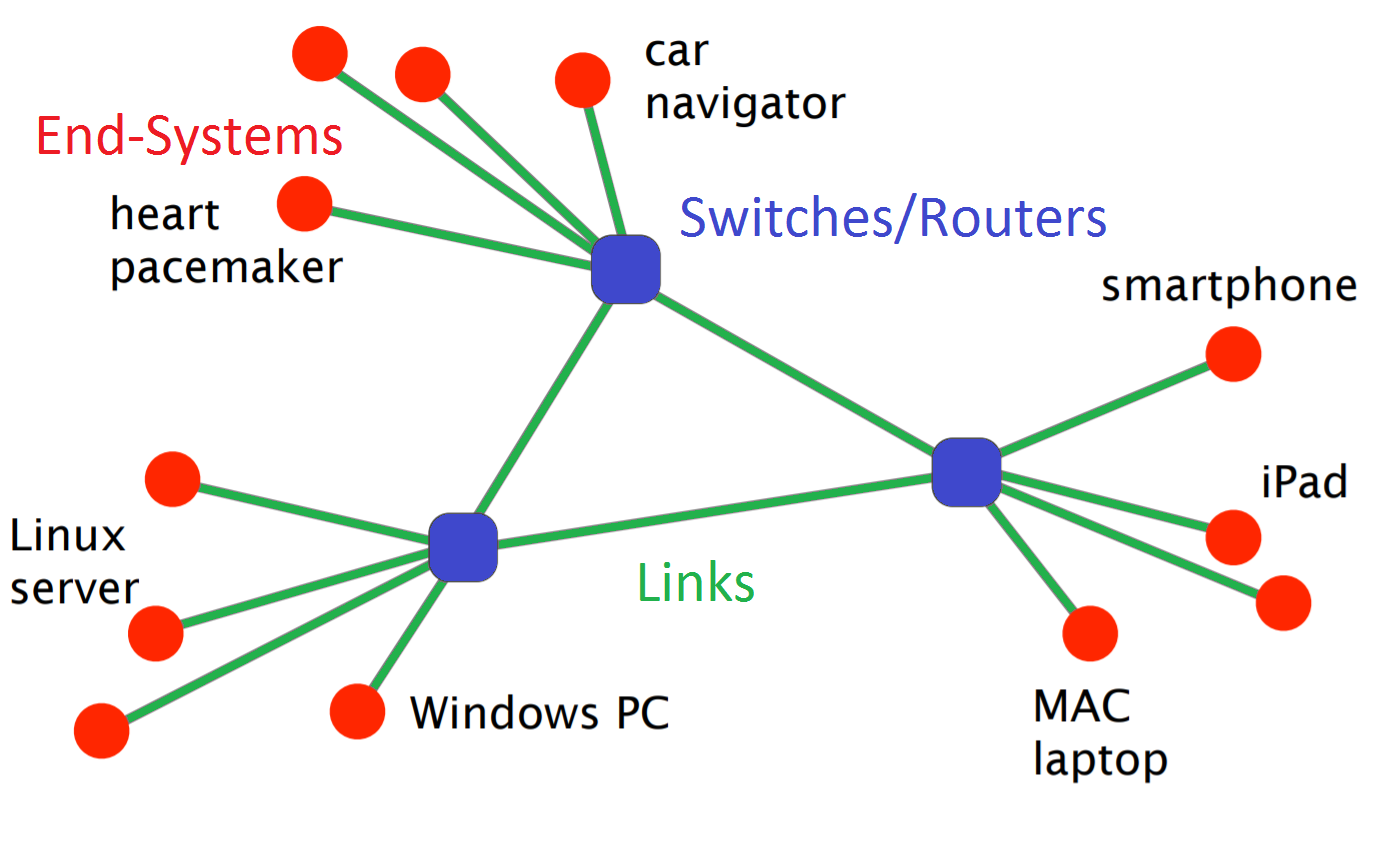
\includegraphics[width= \columnwidth]{images/Overview/network_components.png}
				The internet is a network of networks. The Internet Service Providers (ISP) provide internet to their customers.\\
				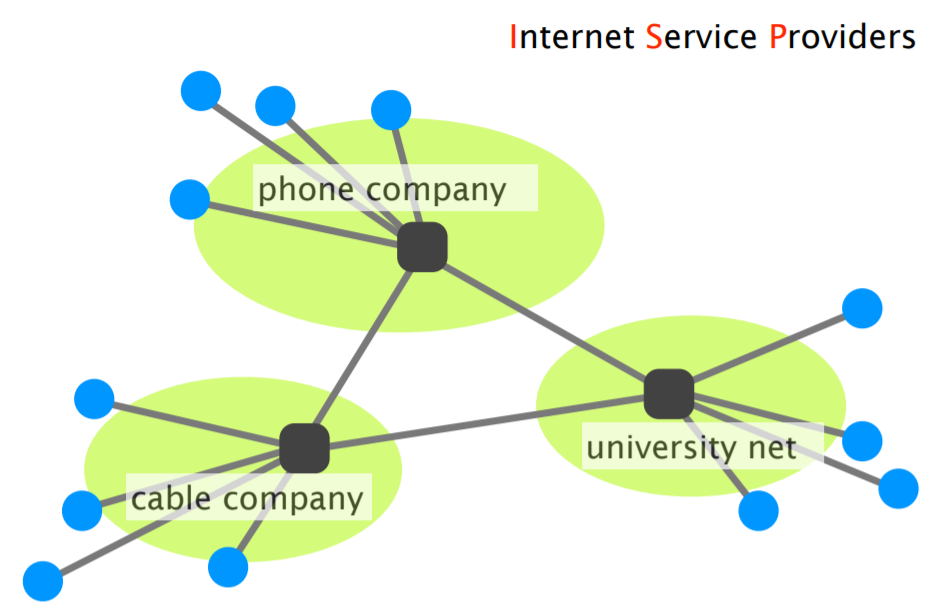
\includegraphics[width= \columnwidth]{images/Overview/ISP.png}
				\columnbreak
			
				There exists a huge amount of \textbf{access technologies: }
				\begin{itemize}[noitemsep]
					\item \textbf{Ethernet} $\vert$ most common, symmetric (Up- and Down-stream same bandwidth)
					\item \textbf{DSL} $\vert$ phone lines, asymmetric (Up- and Down-stream NOT same bandwidth)
					\item \textbf{CATV} $\vert$ via cable TV, shared
					\item \textbf{Cellular} $\vert$ Smart phones 
					\item \textbf{Satellite} $\vert$ remote areas
					\item \textbf{FTTH} $\vert$ fiber to the home
					\item \textbf{Fibers} $\vert$ Internet backbone 
					\item \textbf{Infiniband} $\vert$ High performance computing 
				\end{itemize}
			\subsection{How is it shared?}
				So far we discussed the "last mile" of the Internet.\\
				3 must-have \textbf{requirements} of a good network topology: 
				\begin{itemize}
					\item \textbf{Tolerate failure} $\vert$ several path between src and dst.
					\item \textbf{Sharing to be feasible (praktikabel) \& cost effective } $\vert$ not too much links 
					\item \textbf{Adequate per-node capacity} $\vert$ not to few links 
				\end{itemize}
				The Design of the Internet is a mix of full-mesh, chain and bus which is an optimization of the above requirements. This topology is called a \textbf{switched network}.
				\vspace{-0.5cm}
				%\vspace{-\topsep}
				\begin{itemize}[noitemsep,topsep=0pt]
					\item \textcolor{ForestGreen}{Advantages:}
					\begin{itemize}
						\item \textcolor{ForestGreen}{Sharing and per-node capacity can be adapted to fit the network needs.}
					\end{itemize} 
					\item \textcolor{Red}{Disadvantages:}
					\begin{itemize}
						\item \textcolor{Red}{Require smart devices to perform; forwarding, routing, resource allocation (Zuweisung) }
					\end{itemize} 
				\end{itemize} 
				In a switched network links and switches are shared between flows.
				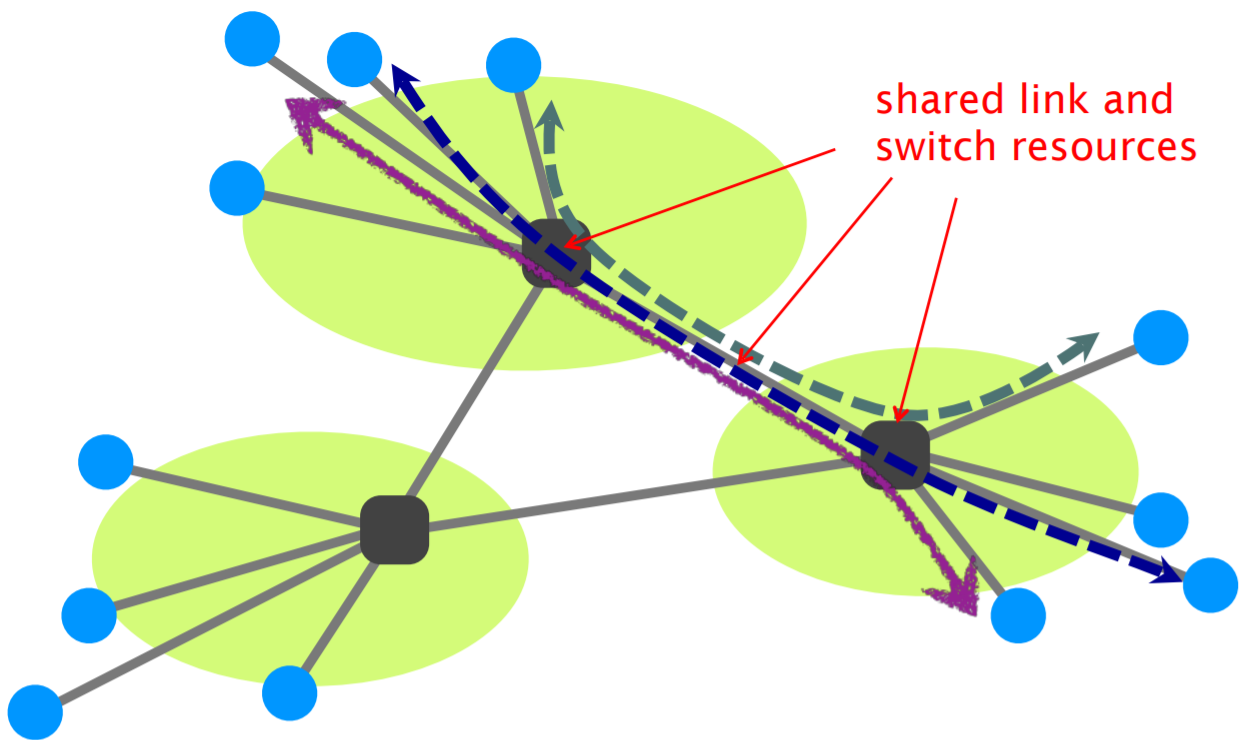
\includegraphics[width= \columnwidth]{images/Overview/link_switch_sharing.png}
				\columnbreak
				
				There exist two approaches of sharing, both are examples of statistical multiplexing: 
				\begin{itemize}
					\item \textcolor{red}{\textbf{Reservation}}\\
						  principle: reserve needed bandwidth in advance\\
						  multiplexing: at the flow-level\\
						  implementation.: circuit-switching  
					\item \textcolor{red}{\textbf{On-demand}}\\
						  principle: send data when you need\\
						  multiplexing: at the packet-level\\
						  implementation.: packet-switching
				\end{itemize}
				\textbf{Circuit-Switching:}
				\vspace{-0.5cm}
				\begin{itemize}[noitemsep]
					\item Relies on the Resource Reservation Protocol.
					\item The efficiency depends on how utilized the circuit is once established. The circuit can be mostly idle or just be used for a small amount of time (bad).
					\item It doesn't route around trouble 
				\end{itemize}
				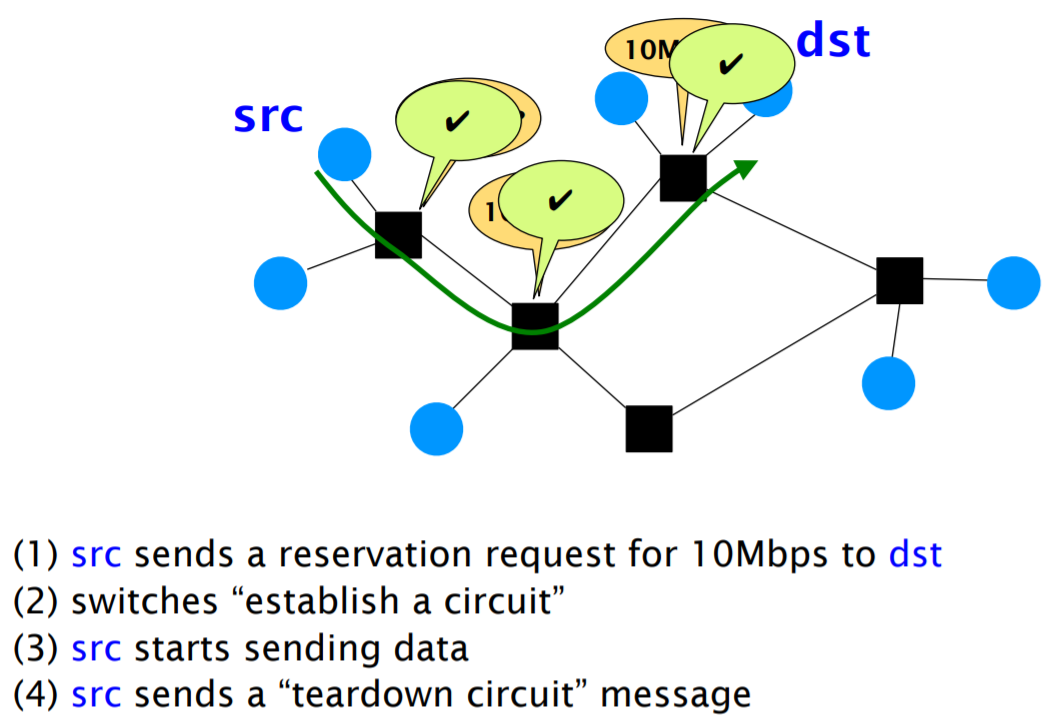
\includegraphics[width=\columnwidth]{images/Overview/circuit_switching.png}
				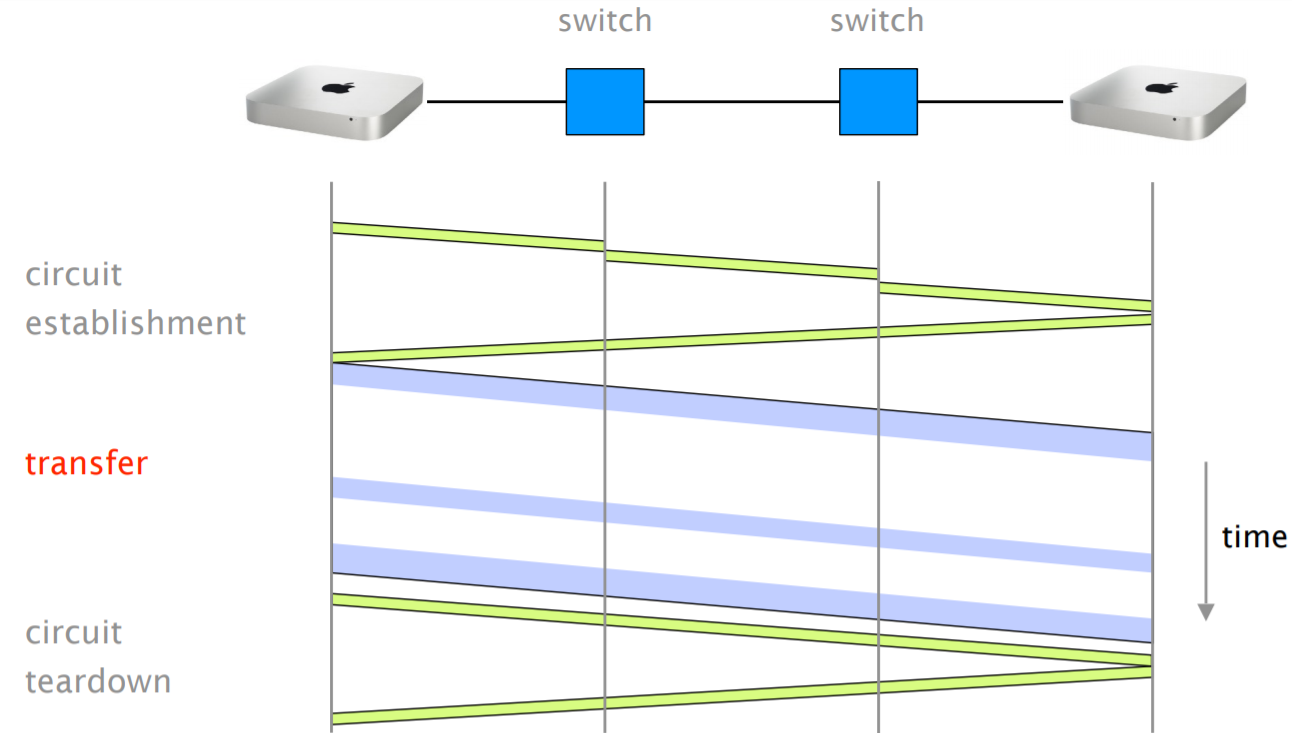
\includegraphics[width=\columnwidth]{images/Overview/circuit_switching_transfer.png}
				\begin{itemize}[noitemsep]
					\item \textcolor{ForestGreen}{Advantages:}
					\begin{itemize}
						\item \textcolor{ForestGreen}{Predictable performance} 
						\item \textcolor{ForestGreen}{Simple \& fast switching (once circuit established)}
					\end{itemize}
					\item \textcolor{red}{Disadvantages:}
					\begin{itemize}
						\item \textcolor{red}{Inefficient if traffic is bursty or short}
						\item \textcolor{red}{Complex circuit setup/teardown (adds delay to transfer)}
						\item \textcolor{red}{Requires new circuit upon failure}
					\end{itemize} 
				\end{itemize}
				\columnbreak
				
				\textbf{Packet-Switching:}
				\vspace{-0.2cm}
				\begin{itemize}[noitemsep]
					\item Data transfer is done using independent packets 
					\item Since packets are not coordinated, they can clash with each other \
					\item To absorb transient overload, packet switching relies on buffers 
					\item It routes around trouble on the fly
				\end{itemize}
				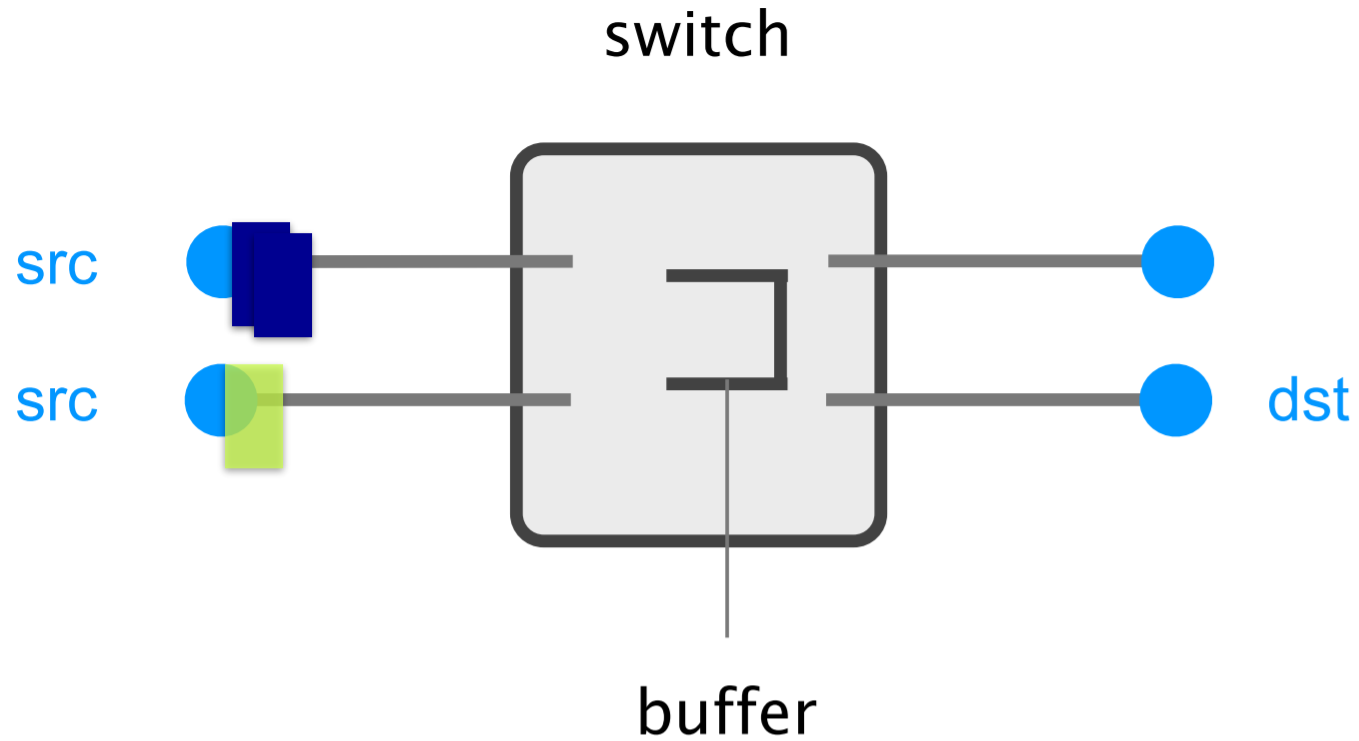
\includegraphics[width=\columnwidth]{images/Overview/packet_switching_buffer.png}
				\begin{itemize}[noitemsep]
					\item \textcolor{ForestGreen}{Advantages:}
					\begin{itemize}
						\item \textcolor{ForestGreen}{Efficient use of resources} 
						\item \textcolor{ForestGreen}{Simpler to implement}
						\item \textcolor{ForestGreen}{Route around trouble}
					\end{itemize}
					\item \textcolor{red}{Disadvantages:}
					\begin{itemize}
						\item \textcolor{red}{unpredictable performance}
						\item \textcolor{red}{Requires buffer management and congestion (Stau) Control}
					\end{itemize} 
				\end{itemize}
				Packet-switching beats circuit-switching with respect to \textbf{resiliency} (robustness) and \textbf{efficiency}. 
				
\includegraphics[width=\columnwidth]{images/Overview/internet_loves_packets.png}
			\newpage
			
			\subsection{How is it organized?}
				The Internet has a hierarchical structure and consists of about 60'000 networks: 
				\begin{itemize}[noitemsep]
					\item \textbf{Tier-1} (international)
					\begin{itemize}
						\item have no provider 
						\item $\approx$12 networks
					\end{itemize}
					\item \textbf{Tier-2} (national)
					\begin{itemize}
						\item provide transit to Tier-3s
						\item have at least 1 provider 
						\item $\approx$1'000s networks 	
					\end{itemize}
					\item \textbf{Tier-3} (local)
					\begin{itemize}
						\item do not provide any transit
						\item have at least one provider
						\item 85-90\% 
					\end{itemize}
				\end{itemize}
				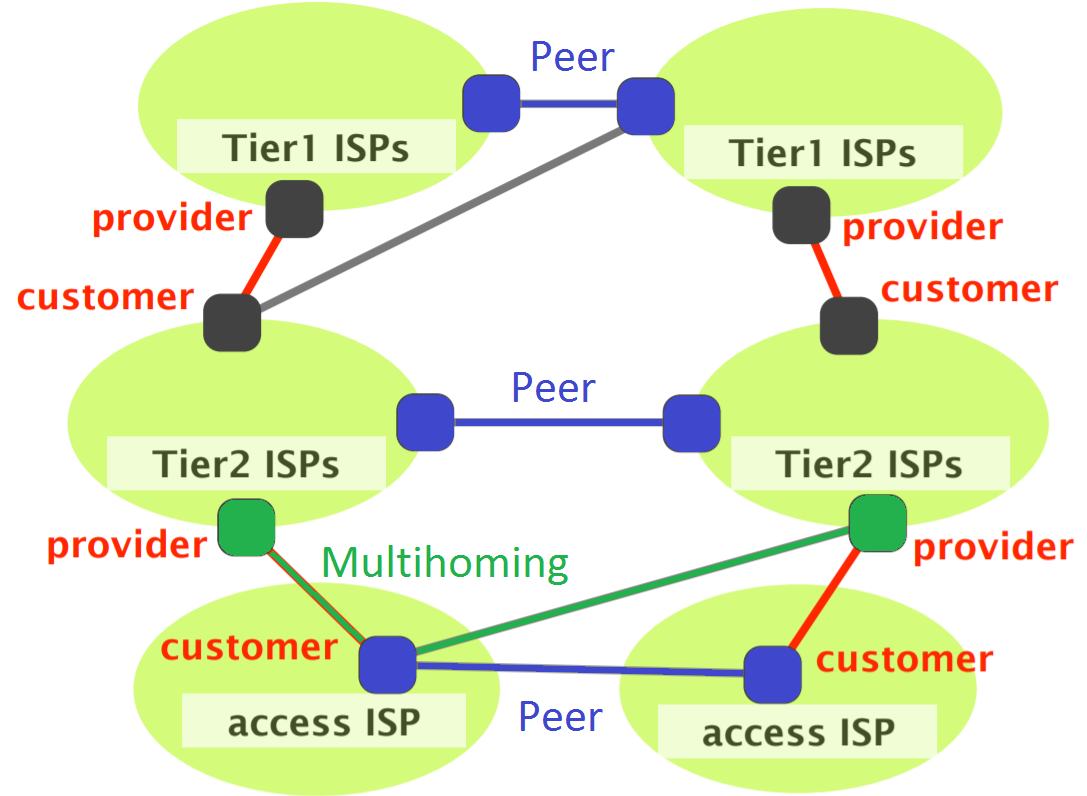
\includegraphics[width=\columnwidth]{images/Overview/hirarchy.png}
				Some networks have an incentive (Anreiz) to connect directly, to reduce their bill with their own provider (direct traffic flow between them). This is known as \textcolor{Blue}{\textbf{peering}}
	\end{multicols*}
	\setcounter{secnumdepth}{2}
\end{document}

